\documentclass[CT4S-EN-RU]{subfiles}

\begin{document}

\section{\caseENGRUS{Monads}{ / }{Монады}}\label{sec:monads}

\begin{blockENG}
Monads would probably not have been invented without category theory, but they have been quite useful in formalizing algebra, calculating invariants of topological spaces, and imbedding non-functional operations into functional programming languages. We will mainly discuss monads in terms of how they can help us make modeling contexts explicit, and in so doing allow us to simplify the language we use in the model.
\end{blockENG}

\begin{blockRUS}
\end{blockRUS}

\begin{blockENG}
Much of the following material on monads is taken from \cite{Sp3}.
\end{blockENG}

\begin{blockRUS}
\end{blockRUS}

%%%% Subsection %%%%

\subsection{\caseENGRUS{Monads formalize context}{ / }{Монады формализуют контекст}}

\begin{blockENG}
Monads can formalize assumptions about the way one will do business throughout a domain. For example, suppose that we want to consider functions that do not have to return a value for all inputs.\index{monad!formalizing context}\index{context} Such {\em partial functions}\index{partial functions} can be composed. Indeed, given a partial function $f\taking A\to B$ and a partial function $g\taking B\to C,$ one gets a partial function $g\circ f\taking A\to C$ in an obvious way.
\end{blockENG}

\begin{blockRUS}
\end{blockRUS}

\begin{blockENG}
Here we are drawing arrows as though we are talking about functions, but there is an implicit context in which we are actually talking about partial functions. Monads allow us to write things in the “functional” way while holding the underlying context. What makes them useful is that the notion of {\em context} we are using here is made formal.
\end{blockENG}

\begin{blockRUS}
\end{blockRUS}

\begin{exampleENG}[Partial functions]\label{ex:partial function monad}\index{a monad!partial functions}\index{partial function}\index{a monad!maybe}
Partial functions can be modeled by ordinary functions, if we add a special “no answer” element to the codomain. That is, the set of partial functions $A\to B$ is in one-to-one correspondence with the set of ordinary functions $A\to B\sqcup\singleton.$ For example, suppose we want to model the partial function $f(x):=\frac{1}{x^2-1}\taking\RR\to\RR$ in this way, we would use the function 
$$f(x):=\begin{cases}
\frac{1}{x^2-1}&\tn{if } x\neq -1 \tn{ and } x\neq 1,\\
\smiley&\tn{if } x=-1,\\
\smiley&\tn{if } x= 1.
\end{cases}
$$
An ordinary function $f\taking A\to B$ can be considered a partial function because we can compose with the inclusion 
\begin{align}\label{dia:first eta}
B\to B\sqcup\singleton
\end{align}

But how do we compose two partial functions written in this way? Suppose $f\taking A\to B\sqcup\singleton$ and $g\taking B\to C\sqcup\singleton$ are functions. First form a new function 
\begin{align}\label{dia:first monad}
g':=g\sqcup\singleton\taking B\sqcup\singleton\to C\sqcup\singleton\sqcup\singleton
\end{align}
then compose to get $(g'\circ f)\taking A\to C\sqcup\singleton\sqcup\singleton,$ and finally send both $\smiley$'s to the same element by composing with 
\begin{align}\label{dia:first mu}
C\sqcup\singleton\sqcup\singleton\to C\sqcup\singleton.
\end{align}

What does this mean? Every element $a\in A$ is sent by $f$ to either an element $b\in B$ or “no answer”. If it has an answer $f(a)\in B,$ this is either sent by $g$ to an element $g(f(a))\in C$ or to “no answer”. We get a partial function $A\to C$ by sending $a$ to $g(f(a))$ if possible or to “no answer” if it gets stopped along the way.

This monad is sometimes called the {\em maybe monad} in computer science, because a partial function $f\taking A\to B$ takes every element of $A$ and either outputs just an element of $B$ or outputs nothing; more succinctly, it outputs a “maybe $B$”.
\end{exampleENG}

\begin{exampleRUS}[Partial functions]\label{ex:partial function monad}\index{a monad!partial functions}\index{partial function}\index{a monad!maybe}
\end{exampleRUS}

\begin{applicationENG}\label{app:experimenter matters}
\href{http://en.wikipedia.org/wiki/Observer-expectancy_effect}{\text Experiments are supposed to be performed objectively}, but suppose we imagine that changing the person who performs the experiment, say in psychology, may change the outcome. Let $A$ be the set of experimenters, let $X$ be the parameter space for the experimental variables (e.g. $X=\tn{Age}\times\tn{Income}$) and let $Y$ be the observation space (e.g. $Y=\tn{propensity for violence}$). Then whereas we want to think of such an experiment as telling us about a function $f\taking X\to Y,$ we may want to make some of the context explicit by including information about who performed the experiment. That is, we are really finding a function $f\taking X\times A\to Y.$ 

However, it may be the case that even ascertaining someones age or income, which is done by asking that person, is subject to who in $A$ is doing the asking, and so we again want to consider the experimenter as part of the equation. In this case, we can use a monad to hide the fact that everything in sight is assumed to be influenced by $A.$ In other words, we want to announce once and for all our modeling context—that every observable is possibly influenced by the observer—so that it can recede into the background.

We will return to this in Examples~\ref{ex:experimenter matters 2} and~\ref{ex:experimenter matters 3}.
\end{applicationENG}

\begin{applicationRUS}\label{app:experimenter matters}
\end{applicationRUS}

%%%% Subsection %%%%

\subsection{\caseENGRUS{Definition and examples}{ / }{Определение и примеры}}

\begin{blockENG}
What aspects of Example~\ref{ex:partial function monad} are really about monads, and what aspects are just about partial functions in particular? It is a functor and a pair of natural transformations that showed up in (\ref{dia:first monad}), (\ref{dia:first eta}), and (\ref{dia:first mu}). In this section we will give the definition and a few examples. We will return to our story about how monads formalize context in Section~\ref{sec:kleisli}.
\end{blockENG}

\begin{blockRUS}
\end{blockRUS}

\begin{definitionENG}[Monad]\label{def:monad}\index{monad}\index{monad!on $\Set$}
A {\em monad on $\Set$} is defined as follows: One announces some constituents (A. functor, B. unit map, C. multiplication map) and asserts that they conform to some laws (1. unit laws, 2. associativity law). Specifically, one announces
\begin{enumerate}[A.]
\item a functor $T\taking\Set\to\Set,$
\item a natural transformation $\eta\taking\id_{\Set}\to T,$ and 
\item a natural transformation $\mu\taking T\circ T\to T$
\end{enumerate}
We sometimes refer to the functor $T$ as though it were the whole monad; we call $\eta$ the {\em unit map} and we call $\mu$ the {\em multiplication map}. One asserts that the following laws hold:
\begin{enumerate}[1.]
\item The following diagrams of functors $\Set\to\Set$ commute:
\begin{align*}
\xymatrix@=30pt{T\circ\id_\Set\ar[r]^-{\id_T\diamond\eta}\ar[dr]_{=}&T\circ T\ar[d]^\mu\\&T}\hspace{1in}
\xymatrix@=30pt{\id_\Set\circ T\ar[r]^-{\eta\diamond\id_T}\ar[dr]_=&T\circ T\ar[d]^\mu\\&T}
\end{align*}
\item The following diagram of functors $\Set\to\Set$ commutes:
\begin{align*}
\xymatrix@=30pt{T\circ T\circ T\ar[r]^-{\mu\diamond\id_T}\ar[d]_-{\id_T\diamond\mu}&T\circ T\ar[d]^\mu\\T\circ T\ar[r]_\mu&T}\end{align*}
\end{enumerate}
\end{definitionENG}

\begin{definitionRUS}[Monad]\label{def:monad}\index{monad}\index{monad!on $\Set$}
\end{definitionRUS}

\begin{exampleENG}[List monad]\label{ex:monad}\index{a monad!List}
We now go through Definition~\ref{def:monad} using what is called the $\List$ monad.\index{list} The first step is to give a functor $\List\taking\Set\to\Set,$ which we did in Example~\ref{ex:free monoid}. Recall that if $X=\{p,q,r\}$ then $\List(X)$ includes the empty list $[\;],$ singleton lists, such as $[p],$ and any other list of elements in $X,$ such as $[p,p,r,q,p].$ Given a function $f\taking X\to Y,$ one obtains a function $\List(f)\taking\List(X)\to\List(Y)$ by entry-wise application of $f.$

As a monad, the functor $\List$ comes with two natural transformations, a unit map $\eta$ and a multiplication map $\mu.$ Given a set $X,$ the unit map $\eta_X\taking X\to\List(X)$ returns singleton lists as follows
$$\xymatrix@=.5pt{
&X\ar[rr]^{\eta_X}&\hspace{1.4in}&\List(X)\\
\ar@{..}[rrr]+<.3in,0pt>&&&\\\\\\
&p\ar@{|->}[rr]&&[p]\\
&q\ar@{|->}[rr]&&[q]\\
&r\ar@{|->}[rr]&&[r]}$$
Given a set $X,$ the multiplication map $\mu_X\taking\List(\List(X))\to\List(X)$ flattens lists of lists as follows.
$$\xymatrix@=.5pt{
&\List(\List(X))\ar[rr]^{\mu_X}&\hspace{.7in}&\List(X)\\
\ar@{..}[rrr]+<.6in,0pt>&&&\\\\\\
&\big[[q, p, r], [], [q, r, p, r], [r]\big]\ar@{|->}[rr]&&[q, p, r, q, r, p, r, r]}$$
The naturality of $\eta$ and $\mu$ just mean that these maps work appropriately well under term-by-term replacement by a function $f\taking X\to Y.$ Finally the three monad laws from Definition~\ref{def:monad} can be exemplified as follows:
$$\xymatrix@=30pt{[p, q, q]\ar@{|->}[r]^-{\id_\List\circ\eta}\ar@{=}[rd]&\big[[p], [q], [q]\big]\ar@{|->}[d]^\mu\\&[p, q, q]}\hspace{.8in}
\xymatrix@=30pt{[p, q, q]\ar@{|->}[r]^-{\eta\circ\id_\List}\ar@{=}[rd]&\big[[p, q, q]\big]\ar@{|->}[d]^\mu\\&[p,q,q]}$$
\vspace{.1in}
$$\xymatrix@=30pt{\Big[\big[[p, q], [r]\big], \big[[], [r, q, q]\big]\Big]\ar@{|->}[r]^-{\mu\circ\id_\List}\ar@{|->}[d]_{\id_\List\circ\mu}&\big[[p, q], [r], [], [r, q, q]\big]\ar@{|->}[d]^\mu\\\big[[p, q, r], [r, q, q]\big]\ar@{|->}[r]_\mu&[p, q, r, r, q,q]}$$
\end{exampleENG}

\begin{exampleRUS}[List monad]\label{ex:monad}\index{a monad!List}
\end{exampleRUS}

\begin{exerciseENG}\label{exc:power set monad}
Let $\PP\taking\Set\to\Set$ be the powerset functor, so that given a function $f\taking X\to Y$ the function $\PP(f)\taking\PP(X)\to\PP(Y)$ is given by taking images.
\sexc Make sense of the following statement: “with $\eta$ defined by singleton subsets and with $\mu$ defined by union, $\top:=(\PP,\eta,\mu)$ is a monad”.
\item  With $X=\{a,b\},$ write down the function $\eta_X$ as a 2-row, 2-column table, and write down the function $\mu_X$ as a 16-row, 2-column table (you can stop after 5 rows if you fully get it).
\item Check that you believe the monad laws from Definition~\ref{def:monad}.
\endsexc
\end{exerciseENG}

\begin{exerciseRUS}\label{exc:power set monad}
\end{exerciseRUS}

\begin{exampleENG}[Partial functions as a monad]\label{ex:partial functions as monad}
Here is the monad for partial functions. The functor $T\taking\Set\to\Set$ sends a set $X$ to the set $X\sqcup\singleton.$ Clearly, given a function $f\taking X\to Y$ there is an induced function $f\sqcup\singleton\taking X\sqcup\singleton\to Y\sqcup\singleton,$ so this is a functor. The natural transformation $\eta\taking\id\to T$ is given on a set $X$ by the component function $$\eta_X\taking X\to X\sqcup\singleton$$ that includes $X\inj X\sqcup\singleton.$ Finally, the natural transformation $\mu\taking T\circ T\to T$ is given on a set $X$ by the component function $$\mu_X\taking X\sqcup\singleton\sqcup\singleton\too X\sqcup\singleton$$ that collapses both copies of $\smiley.$
\end{exampleENG}

\begin{exampleRUS}[Partial functions as a monad]\label{ex:partial functions as monad}
\end{exampleRUS}

\begin{exerciseENG}\label{exc:exceptions}
Let $E$ be a set, elements we will refer to as {\em exceptions}\index{exceptions}\index{a monad!exceptions}. We imagine that a function $f\taking X\to Y$ either outputs a value or one of these exceptions, which might be things like “overflow!” or “division by zero!”, etc. Let $T\taking\Set\to\Set$ be the functor $X\mapsto X\sqcup E.$ Follow Example~\ref{ex:partial functions as monad} and come up with a unit map $\eta$ and a multiplication map $\mu$ for which $(T,\eta,\mu)$ is a monad.
\end{exerciseENG}

\begin{exerciseRUS}\label{exc:exceptions}
\end{exerciseRUS}

\begin{exampleENG}\label{ex:experimenter matters 2}
Fix a set $A.$ Let $T\taking\Set\to\Set$ be given by $T(X)=X^A=\Hom_\Set(A,X)$; this is a functor. For a set $X,$ let $\eta_X\taking X\to T(X)$ be given by the constant function, $x\mapsto c_x\taking A\to X$ where $c_x(a)=x$ for all $a\in A.$ To specify a function
$$\mu_X\taking\Hom_\Set(A,T(X))\to\Hom_\Set(A,X),$$ we curry and need a function $A\times\Hom_\Set(A,T(X))\to X.$ We have an evaluation function (see Exercise~\ref{exc:evaluation}) $ev\taking A\times\Hom_\Set(A,T(X))\to T(X),$ and we have an identity function $\id_A\taking A\to A,$ so we have a function $(\id_A\times ev)\taking A\times\Hom_\Set(A,T(X))\too A\times T(X).$ Composing that with another evaluation function $A\times\Hom_\Set(A,X)\to X$ yields our desired $\mu_X.$ Namely, for all $b\in A$ and $f\in\Hom(A,T(X))$ we have
$$\mu_X(f)(b)=f(b)(b).$$
\end{exampleENG}

\begin{exampleRUS}\label{ex:experimenter matters 2}
\end{exampleRUS}

\begin{remarkENG}\index{monad!on $\Grph$}\index{a monad!$\Paths$}
Monads can be defined on categories other than $\Set.$ In fact, for any category $\mcC$ one can take Definition~\ref{def:monad} and replace every occurrence of $\Set$ with $\mcC$ and obtain the definition for monads on $\mcC.$ We have actually seen a monad $(\Paths,\eta,\mu)$ on the category $\Grph$ of graphs before, namely in Examples~\ref{ex:graph to paths} and~\ref{ex:concat paths of paths}. That is, $\Paths\taking\Grph\to\Grph,$ which sends a graph to its paths-graph\index{graph!paths-graph} is the functor part. The unit map $\eta$ includes a graph into its paths-graph using the observation that every arrow is a path of length 1. And the multiplication map $\mu$ concatenates paths of paths. The Kleisli category of this monad (see Definition~\ref{def:kleisli}) is used, e.g. in (\ref{dia:kleisli comp in graph}) to define morphisms of database schemas.
\end{remarkENG}

\begin{remarkRUS}\index{monad!on $\Grph$}\index{a monad!$\Paths$}
\end{remarkRUS}

%%%% Subsection %%%%

\subsection{\caseENGRUS{Kleisli category of a monad}{ / }{Категория Клейсли монады}}\label{sec:kleisli}

\begin{blockENG}
Given a monad $\top:=(T,\eta,\mu),$ we can form a new category $\Kls(\top).$
\end{blockENG}

\begin{blockRUS}
\end{blockRUS}

\begin{definitionENG}\label{def:kleisli}\index{category!Kleisli}\index{Kleisli category}\index{monad!Kleisli category of}
Let $\top=(T,\eta,\mu)$ be a monad on $\Set.$ Form a new category, called the {\em Kleisli category for $\top$}, denoted $\Kls(\top),$ with sets as objects, $\Ob(\Kls(\top)):=\Ob(\Set),$ and with $$\Hom_{\Kls(\top)}(X,Y):=\Hom_\Set(X,T(Y))$$ for sets $X,Y.$ The identity morphism $\id_X\taking X\to X$ in $\Kls(\top)$ is given by $\eta\taking X\to T(X)$ in $\Set.$ The composition of morphisms $f\taking X\to Y$ and $g\taking Y\to Z$ in $\Kls(\top)$ is given as follows. Writing them as functions, we have $f\taking X\to T(Y)$ and $g\taking Y\to T(Z).$ The first step is to apply the functor $T$ to $g,$ giving $T(g)\taking T(Y)\to T(T(Z)).$ Then compose with $f$ to get $T(g)\circ f\taking X\to T(T(Z)).$ Finally, compose with $\mu_Z\taking T(T(Z))\to T(Z)$ to get the required function $X\to T(Z).$ The associativity of this composition formula follows from the associativity law for monads.
\end{definitionENG}

\begin{definitionRUS}\label{def:kleisli}\index{category!Kleisli}\index{Kleisli category}\index{monad!Kleisli category of}
\end{definitionRUS}

\begin{exampleENG}
Recall the monad $\top$ for partial functions, $T(X)=X\sqcup\singleton,$ from Example~\ref{ex:partial functions as monad}. The Kleisli category $\Kls(\top)$ has sets as objects, but a morphism $f\taking X\to Y$ means a function $X\to Y\sqcup\singleton,$ i.e a partial function. Given another morphism $g\taking Y\to Z,$ the composition formula in $\Kls(\top)$ ensures that $g\circ f\taking X\to Z$ has the appropriate behavior.

Note how this monad allows us to make explicit our assumption that all functions are partial, and then hide it away from our notation.
\end{exampleENG}

\begin{exampleRUS}
\end{exampleRUS}

\begin{remarkENG}\label{rem:ordinary are kleisli}
For any monad $\top=(T,\eta,\mu)$ on $\Set,$ there is a functor $i\taking \Set\to\Kls(\top)$ given as follows. On objects we have $\Ob(\Kls(\top))=\Ob(\Set),$ so take $i=\id_{\Ob(\Set)}.$ Given a morphism $f\taking X\to Y$ in $\Set,$ we need a morphism $i(f)\taking X\to Y$ in $\Kls(\top),$ i.e. a function $i(f)\taking X\to T(Y).$ We assign $i(f)$ to be the composite $X\To{f}Y\To{\eta}T(Y).$ The functoriality of this mapping follows from the unit law for monads.

The point is that any ordinary function (morphism in $\Set$) has an interpretation as a morphism in the Kleisli category of any monad. More categorically, there is a functor $\Set\to\Kls(\top).$
\end{remarkENG}

\begin{remarkRUS}\label{rem:ordinary are kleisli}
\end{remarkRUS}

\begin{exampleENG}\label{ex:experimenter matters 3}
In this example we return to the setting laid out by Application~\ref{app:experimenter matters} where we had a set $A$ of experimenters and assumed that the person doing the experiment may affect the outcome. We use the monad $\top=(T,\eta,\mu)$ from Example~\ref{ex:experimenter matters 2} and hope that $\Kls(\top)$ will conform to our understanding of how to manage the affect of the experimenter on data.

The objects of $\Kls(\top)$ are ordinary sets, but a map $f\taking X\to Y$ in $\Kls(\top)$ is a function $X\to Y^A.$ By currying this is the same as a function $X\times A\to Y,$ as desired. To compose $f$ with $g\taking Y\to Z$ in $\Kls(\top),$ we follow the formula. It turns out to be equivalent to the following. We have a function $X\times A\to Y$ and a function $Y\times A\to Z.$ Modifying the first slightly, we have a function $X\times A\to Y\times A,$ by identity on $A,$ and we can now compose to get $X\times A\to Z.$

What does this say in terms of experimenters affecting data gathering? It says that if we work within $\Kls(\top)$ then we will be able to assume that the experimenter is being taken into account; all proposed functions $X\to Y$ are actually functions $A\times X\to Y.$ The natural way to compose these experiments is that we only consider the data from one experiment to feed into another if the experimenter is the same in both experiments.
\footnote{This requirement seems a bit stringent, but it can be mitigated in a variety of ways. One such way is to notice that by Remark~\ref{rem:ordinary are kleisli} that we have not added any requirement, because any old way of doing business yields a valid new way of doing business (we just say “every experimenter would get the same result”). Another way would be to hand off the experiment results to another person, who could carry it forward (see Example~\ref{ex:preorder monad}).}
\end{exampleENG}

\begin{exampleRUS}\label{ex:experimenter matters 3}
\end{exampleRUS}

\begin{exerciseENG}\label{exc:kleisli powerset relations}
In Exercise~\ref{exc:power set monad} we discussed the power set monad $\top=(\PP,\eta,\mu).$
\sexc Can you find a way to relate the morphisms in $\Kls(\top)$ to relations? That is, given a morphism $f\taking A\to B$ in $\Kls(\top),$ is there a natural way to associate to it a relation $R\ss A\times B?$
\item How does the composition formula in $\Kls(\top)$ relate to the composition of relations given in Definition~\ref{def:composite span}?
\footnote{Actually, Definition~\ref{def:composite span} is about composing spans, but a relation $R\ss A\times B$ is a kind of span, $R\to A\times B.$}
\endsexc
\end{exerciseENG}

\begin{exerciseRUS}\label{exc:kleisli powerset relations}
\end{exerciseRUS}

\begin{exerciseENG}
Let $\top=(\PP,\eta,\mu)$ be the power set monad. The category $\Kls(\top)$ is closed under binary products, i.e. every pair of objects $A,B\in\Ob(\Kls(\top))$ have a product in $\Kls(\top).$ What is the product of $A=\{1,2,3\}$ and $B=\{a,b\}?$
\end{exerciseENG}

\begin{exerciseRUS}
\end{exerciseRUS}

\begin{exerciseENG}
Let $\top=(\PP,\eta,\mu)$ be the power set monad. The category $\Kls(\top)$ is closed under binary coproducts, i.e. every pair of objects $A,B\in\Ob(\Kls(\top))$ have a coproduct in $\Kls(\top).$ What is the coproduct of $A=\{1,2,3\}$ and $B=\{a,b\}?$
\end{exerciseENG}

\begin{exerciseRUS}
\end{exerciseRUS}

\begin{exampleENG}\label{ex:preorder monad}
Let $A$ be any preorder. We speak of $A$ throughout this example as though it was the linear order given by time because this is a nice case, however the mathematics works for any $A\in\Ob(\PrO).$ 

There is a monad $\top=(T,\eta,\mu)$ that captures the idea that a function $f\taking X\to Y$ occurs in the context of time in the following sense: The output of $f$ is determined not only by the element $x\in X$ on which it is applied but also by the time at which it was applied to $x$; and the output of $f$ occurs at another time, which is not before the time of input.

The functor part of the monad is given on $X\in\Ob(\Set)$ by
$$T(X)=\{p\taking A\to A\times X\|\tn{ if } p(a)=(a',x)\tn{ then } a'\geq a\}.$$
The unit $\eta_X\taking X\to T(X)$ sends $x$ to the function $a\mapsto (a,x).$ The multiplication map $\mu_X\taking T(T(X))\to T(X)$ is roughly described as follows. If for every $a\in A$ you have a later element $a'\geq a$ and a function $p\taking A\to A\times X$ that takes elements of $A$ to later elements of $A$ and values of $X,$ then $p(a')$ is a still later element of $A$ and a value of $X,$ as desired.

Morphisms in the Kleisli category $\Kls(\top)$ can be curried to be functions $f\taking A\times X\to A\times Y$ such that if $f(a,x)=(a',y)$ then $a'\geq a.$ 
\end{exampleENG}

\begin{exampleRUS}\label{ex:preorder monad}
\end{exampleRUS}

\begin{remarkENG}\label{rem:state monad}
One of the most important monads in computer science is the so-called {\em state monad}. It is used when one wants to allow a program to mutate state variables (e.g. in the program 
\begin{quote}if $x>4$ then $x:=x+1$ else Print “done”)\end{quote}
$x$ is a state variable. The state monad is a special case of the monad discussed in Example~\ref{ex:preorder monad}. Given any set $A,$ the usual {\em state monad of type $A$} is obtained by giving $A$ the indiscrete preorder (see Example~\ref{ex:discrete and indiscrete}). More explicitly it is a monad with functor part $$X\mapsto (A\times X)^X,$$ and it will be briefly discussed in Example~\ref{ex:currying gives state}.
\end{remarkENG}

\begin{remarkRUS}\label{rem:state monad}
\end{remarkRUS}

\begin{exampleENG}\label{ex:scientific method}
Here we reconsider the image from the front cover of this book, reproduced here.
\begin{center}
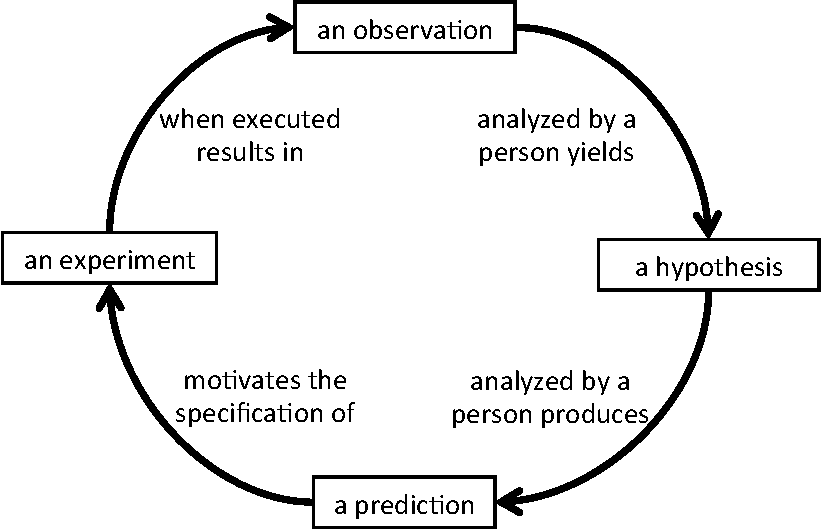
\includegraphics[width=.8\textwidth]{ScientificMethod}
\end{center}

It looks like an olog, and all ologs are database schemas (see Section~\ref{sec:olog as db schema}). But how is “analyzed by a person yields” a function from observations to hypotheses? The very name belies the fact that it is an invalid aspect in the sense of Section~\ref{sec:invalid aspect}, because given an observation there may be more than one hypothesis yielded, corresponding to which person is doing the observing. In fact, all of the arrows in this diagram correspond to some hidden context involving people: the prediction is dependent on who analyzes the hypothesis, the specification of an experiment is dependent on who is motivated to specify it, and experiments may result in different observations by different observers. 

Without monads, the model of science proposed by this olog would be difficult to believe in. But by choosing a monad we can make explicit (and then hide from discourse) our implicit assumption that “of course this is all dependent on which human is doing the science”. The choice of monad is an additional modeling choice. Do we want to incorporate the partial order of time? Do we want the scientist to be modified by each function (i.e. the person is changed when analyzing an observation to yield a hypothesis)? These are all interesting possibilities. 

One reasonable choice would be to use the state monad of type $A,$ where $A$ is the set of scientific models. This implies the following context: every morphism $f\taking X\to Y$ in the Kleisli category of this monad is really a morphism $f\taking X\times A\to Y\times A$; while ostensibly giving a map from $X$ to $Y,$ it is influenced by the scientific model under which it is performed, and its outcome yields a new scientific model. 

Reading the olog in this context might look like this:

\begin{quote}
A hypothesis (in the presence of a scientific model) analyzed by a person produces a prediction (in the presence of a scientific model), which motivates the specification of an experiment (in the presence of a scientific model), which when executed results in an observation (in the presence of a scientific model), which analyzed by a person yields a hypothesis (in the presence of a scientific model).
\end{quote}

The parenthetical statements can be removed if we assume them to always be around, which can be done using the monad above.
\end{exampleENG}

\begin{exampleRUS}\label{ex:scientific method}
\end{exampleRUS}

%% Subsubsection %%

\subsubsection{\caseENGRUS{Relaxing functionality constraint for ologs}{ / }{Ослабление ограничений на функциональность олога}}\label{sec:relaxing ologs}

\begin{blockENG}
In Section~\ref{sec:aspects} we said that every arrow in an olog has to be English-readable as a sentence, and it has to correspond to a function. For example, the arrow 
\begin{align}\label{dia:non-functional but english}
\xymatrix{\fbox{a person}\LA{r}{has}&\fbox{a child}}
\end{align}
comprises an readable sentence, but does not correspond to a function because a person may have no children or more than one child. 
We'll call olog in which every arrow corresponds to a function (the only option proposed so far in the book) a {\em functional olog}. Requiring that ologs be functional as we have been doing, comes with advantages and disadvantages. The main advantage is that creating a functional olog requires more conceptual clarity about the situation, and this has benefits for the olog-creator as well as for anyone to whom he or she tries to explain the situation. The main disadvantage is that creating a functional olog takes more time, and the olog takes up more space on the page.
\end{blockENG}

\begin{blockRUS}
\end{blockRUS}

\begin{blockENG}
In the context of the power set monad (see Exercise~\ref{exc:power set monad}), a morphism $f\taking X\to Y$ between sets $X$ and $Y$ becomes a binary relation on $X$ and $Y,$ rather than a function, as seen in Exercise~\ref{exc:kleisli powerset relations}. So in that context, the arrow in (\ref{dia:non-functional but english}) becomes valid. An olog in which arrows correspond to mere binary relations rather than functions might be called a {\em relational olog}.\index{olog!relational}
\end{blockENG}

\begin{blockRUS}
\end{blockRUS}

%%%% Subsection %%%%

\subsection{\caseENGRUS{Monads in databases}{ / }{Монады в базах данных}}\label{sec:monads in db}

\begin{blockENG}
In this section we discuss how to record data in the presence of a monad. The idea is quite simple. Given a schema (category) $\mcC,$ an ordinary instance is a functor $I\taking\mcC\to\Set.$ But if $\top=(T,\eta,\mu)$ is a monad, then a {\em Kleisli $\top$-instance on $\mcC$} is a functor $J\taking\mcC\to\Kls(\top).$ Such a functor associates to every object $c\in\Ob(\mcC)$ a set $J(c),$ and to every arrow $f\taking c\to c'$ in $\mcC$ a morphism $J(f)\taking J(c)\to J(c')$ in $\Kls(\top).$ How does this look in terms of tables?
\end{blockENG}

\begin{blockRUS}
\end{blockRUS}

\begin{blockENG}
Recall that to represent an ordinary database instance $I\taking\mcC\to\Set,$ we use a tabular format in which every object $c\in\Ob(\mcC)$ is displayed as a table including one ID column and an additional column for every arrow emanating from $c.$ In the ID column of table $c$ were elements of the set $I(c)$ and in the column assigned to some arrow $f\taking c\to c'$ the cells were elements of the set $I(c').$ 
\end{blockENG}

\begin{blockRUS}
\end{blockRUS}

\begin{blockENG}
To represent a {\em Kleisli}\index{database!Kleisli}\index{instance!Kleisli} database instance $J\taking\mcC\to\Kls{\top}$ is similar; we again use a tabular format in which every object $c\in\Ob(\mcC)$ is displayed as a table including one ID column and an additional column for every arrow emanating from $c.$ In the ID column of table $c$ are again elements of the set $J(c)$; however in the column assigned to some arrow $f\taking c\to c'$ are not elements of $J(c')$ but $T$-values in $J(c'),$ i.e. elements of $T(J(c')).$ 
\end{blockENG}

\begin{blockRUS}
\end{blockRUS}

\begin{exampleENG}
Let $\top=(T,\eta,\mu)$ be the monad for partial functions, as discussed in Example~\ref{ex:partial function monad}. Given any schema $\mcC,$ we can represent a Kleisli $\top$-instance $I\taking\mcC\to\Kls(\top)$ in tabular format. To every object $c\in\Ob(\mcC)$ we'll have a set $I(c)$ of rows, and given a column $c\to c'$ every row will produce either a value in $I(c')$ or fail to produce a value; this is the essence of partial functions. We might denote the absence of a value using $\smiley.$

Consider the schema indexing graphs 
$$\mcC:=\fbox{\xymatrix{\LTO{Arrow}\ar@<.5ex>[r]^{src}\ar@<-.5ex>[r]_{tgt}&\LTO{Vertex}}}$$
As we discussed in Section~\ref{sec:graphs as functors}, an ordinary instance on $\mcC$ represents a graph. 
\begin{align*}
I:=\parbox{2in}{\fbox{\xymatrix{\bullet^v\ar[r]^f&\bullet^w\ar@/_1pc/[r]_h\ar@/^1pc/[r]^g&\bullet^x}}}
\hspace{.5in}
\begin{array}{| l || l | l |}\bhline
\multicolumn{3}{|c|}{{\tt Arrow}\;\; (I)}\\\bhline
{\bf ID}&{\bf src}&{\bf tgt}\\\bbhline
f&v&w\\\hline
g&w&x\\\hline
h&w&x\\\bhline
\end{array}
\hspace{.5in}
\begin{array}{| l ||}\bhline
\multicolumn{1}{|c|}{{\tt Vertex}\;\; (I)}\\\bhline
{\bf ID}\\\bbhline
v\\\hline
w\\\hline
x\\\bhline
\end{array}
\end{align*}
A Kleisli $\top$-instance on $\mcC$ represents graphs in which edges can fail to have a source vertex, fail to have a target vertex, or both. 
\begin{align*}
J:=\parbox{2in}{\fbox{\xymatrix{\bullet^v\ar[d]_i\ar[r]^f&\bullet^w\ar@/_1pc/[r]_h\ar@/^1pc/[r]^g&\bullet^x\\&\ar[r]_j&}}}
\hspace{.5in}
\begin{array}{| l || l | l |}\bhline
\multicolumn{3}{|c|}{{\tt Arrow}\;\; (J)}\\\bhline
{\bf ID}&{\bf src}&{\bf tgt}\\\bbhline
f&v&w\\\hline
g&w&x\\\hline
h&w&x\\\hline
i&v&\smiley\\\hline
j&\smiley&\smiley\\\bhline
\end{array}
\hspace{.5in}
\begin{array}{| l ||}\bhline
\multicolumn{1}{|c|}{{\tt Vertex}\;\; (J)}\\\bhline
{\bf ID}\\\bbhline
v\\\hline
w\\\hline
x\\\bhline
\end{array}
\end{align*}
The context of these tables is that of partial functions, so we do not need a reference for $\smiley$ in the vertex table. Mathematically, the morphism $J(src)\taking J({\tt Arrow})\to J({\tt Vertex})$ needs to be a function $J({\tt Arrow})\to J({\tt Vertex})\sqcup\singleton,$ and it is.
\end{exampleENG}

\begin{exampleRUS}
\end{exampleRUS}

\subsubsection{\caseENGRUS{Probability distributions}{ / }{Распределения вероятностей}}

\begin{blockENG}
Let $[0,1]\ss\RR$ denote the set of real numbers between $0$ and $1.$ Let $X$ be a set and $p\taking X\to[0,1]$ a function. We say that $p$ is a {\em finitary probability distribution on $X$} if there exists a finite subset $W\ss X$ such that 
\begin{align}\label{dia:sum to 1}
\sum_{w\in W}p(w)=1,
\end{align} and such that $p(x)>0$ if and only if $x\in W.$ Note that $W$ is unique if it exists; we call it {\em the support of $p$} and denote it $\Supp(p).$ Note also that if $X$ is a finite set then every function $p$ satisfying (\ref{dia:sum to 1}) is a finitary probability distribution on $X.$
\end{blockENG}

\begin{blockRUS}
\end{blockRUS}

\begin{blockENG}
For any set $X,$ let $\Dist(X)$ denote the set of finitary probability distributions on $X.$ It is easy to check that given a function $f\taking X\to Y$ one obtains a function $\Dist(f)\taking\Dist(X)\to\Dist(Y)$ by $\Dist(f)(y)=\sum_{f(x)=y}p(x).$ Thus we can consider $\Dist\taking\Set\to\Set$ as a functor, and in fact the functor part of a monad. Its unit $\eta\taking X\to\Dist(X)$ is given by the Kronecker delta function $x\mapsto \delta_x$ where $\delta_x(x)=1$ and $\delta_x(x')=0$ for $x'\neq x.$ Its multiplication $\mu\taking\Dist(\Dist(X))\to\Dist(X)$ is given by weighted sum: given a finitary probability distribution $w\taking\Dist(X)\to[0,1]$ and $x\in X,$ put $\mu(w)(x)=\sum_{p\in\Supp(w)}w(p)p(x).$ %For details one may consult \cite{Tam}, which goes further into the subject of including probability in databases.
\end{blockENG}

\begin{blockRUS}
\end{blockRUS}

\begin{exampleENG}[Markov chains]\label{ex:markov}\index{Markov chain}\index{a schema!$\Loop$}
Let $\Loop$ be the loop schema, $$\Loop:=\LoopSchema$$ as in Example~\ref{ex:dds}. A $\Dist$-instance on $\Loop$ is equivalent to a time-homogeneous Markov chain. To be explicit, a functor $\delta\taking\Loop\to\Kls{\Dist}$ assigns to the unique object $s\in\Ob(\Loop)$ a set $S=\delta(s),$ which we call the state space, and to $f\taking s\to s$ a function $\delta(f)\taking S\to\Dist(S),$ which sends each element $x\in S$ to some probability distribution on elements of $S.$ For example, the table $\delta$ on the left corresponds to the Markov matrix $M$ on the right below:
\begin{align}
\delta:=
\begin{tabular}{| l || l |}\bhline
\multicolumn{2}{| c |}{\tt{s}}\\\bhline 
{\bf ID}&{\bf f}\\\bbhline
1 & .5(1)+.5(2)\\\hline
2 & 1(2)\\\hline
3 & .7(1)+.3(3)\\\hline
4 & .4(1)+.3(2)+.3(4)\\\bhline
\end{tabular}
\hspace{.5in}
M:=\left(
\begin{array}{cccc}
0.5 & 0.5 & 0 & 0\\
0 & 1 & 0 & 0\\
0.7 & 0 & 0.3 & 0\\
0.4 & 0.3 & 0 &0.3
\end{array}
\right)
\end{align}

As one might hope, for any natural number $n\in\NN$ the map $f^n\taking S\to\Dist(S)$ corresponds to the matrix $M^n,$ which sends an element in $S$ to its probable location after $n$ iterations of the transition map.
\end{exampleENG}

\begin{exampleRUS}[Markov chains]\label{ex:markov}\index{Markov chain}\index{a schema!$\Loop$}
\end{exampleRUS}

\begin{applicationENG}
Every star \href{http://cas.sdss.org/dr6/en/proj/basic/color/fromstars.asp}{emits a spectrum of light}, which can be understood as a distribution on the electromagnetic spectrum. Given an object $B$ on earth, different parts of $B$ will \href{http://en.wikipedia.org/wiki/Absorption_spectroscopy}{absorb radiation} at different rates. Thus $B$ produces a function from the electromagnetic spectrum to distributions of energy absorption. In the context of the probability distributions monad, we can record data on the schema 
$$\xymatrix{\LTO{star}\LA{rr}{emits}&&\LTO{wavelengths}\LA{rr}{absorbed by $B$}&\hspace{.2in}&\LTO{energies}}$$
The composition formula for Kleisli categories is the desired one: to each star we associate the weighted sum of energy absorption rates over the set of wavelengths emitted by the star. 
\end{applicationENG}

\begin{applicationRUS}
\end{applicationRUS}

%%%% Subsection %%%%

\subsection{\caseENGRUS{Monads and adjunctions}{ / }{Монады и сопряжения}}

\begin{blockENG}
There is a strong connection between monads and adjunctions: every adjunction creates a monad, and every monad “comes from” an adjunction. For example, the $\List$ monad (Example~\ref{ex:monad}) comes from the free-forgetful adjunction between sets and monoids
$$\Adjoint{F}{\Set}{\Mon}{U}$$
(see Proposition~\ref{prop:free forgetful monoid}). That is, for any set $X,$ the free monoid on $X$ is $$F(X)=(\List(X),[\;],\plpl),$$ and the underlying set of that monoid is $U(F(X))=\List(X).$ Now it may seem like there was no reason to use monoids at all—the set $\List(X)$ was needed in order to discuss $F(X)$—but it will turn out that the unit $\eta$ and multiplication $\mu$ will come drop out of the adjunction too. First, we discuss the unit and counit of an adjunction.
\end{blockENG}

\begin{blockRUS}
\end{blockRUS}

\begin{definitionENG}\label{def:unit and counit of adjunction}\index{adjunction!unit}\index{adjunction!counit}
Let $\mcC$ and $\mcD$ be categories, and let $L\taking\mcC\to\mcD$ and $R\taking\mcD\to\mcC$ be functors with adjunction isomorphism 
$$\alpha_{c,d}\taking\Hom_\mcD(L(c),d)\Too{\iso}\Hom_\mcC(c,R(d))$$
for any objects $c\in\Ob(\mcC)$ and $d\in\Ob(\mcD).$ The {\em unit} $\eta\taking\id_\mcC\to R\circ L$ (respectively the {\em counit} $\epsilon\taking L\circ R\to\id_\mcD$) are natural transformations defined as follows.

Given an object $c\in\Ob(\mcC),$ we apply $\alpha$ to $\id_{L(c)}\taking L(c)\to L(c)$ to get 
$$\eta_c\taking c\to R\circ L(c);$$ 
similarly given an object $d\in\Ob(\mcD)$ we apply $\alpha^\m1$ to $\id_{R(d)}\taking R(d)\to R(d)$ to get 
$$\epsilon_d\taking L\circ R(d)\to d.$$ 
\end{definitionENG}

\begin{definitionRUS}\label{def:unit and counit of adjunction}\index{adjunction!unit}\index{adjunction!counit}
\end{definitionRUS}

\begin{blockENG}
Below we will show how to use the unit and counit of any adjunction to make a monad. We first walk through the process in Example~\ref{ex:list adjunction makes monad}.
\end{blockENG}

\begin{blockRUS}
\end{blockRUS}

\begin{exampleENG}\label{ex:list adjunction makes monad}
Consider the adjunction $\Adjoint{F}{\Set}{\Mon}{U}$ between sets and monoids. Let $T=U\circ F\taking\Set\to\Set$; this will be the functor part of our monad, and we have $T=\List.$ Then the unit of the adjunction, $\eta\taking\id_\Set\to U\circ F$ is precisely the unit of the monad: for any set $X\in\Ob(\Set)$ the component $\eta_X\taking X\to\List(X)$ is the function that takes $x\in X$ to the singleton
list $[x]\in\List(X).$ The monad also has a multiplication map $\mu_X\taking T(T(X))\to T(X),$ which amounts to flattening a list of lists. This function comes about using the counit $\epsilon,$ as follows 
$$T\circ T=U\circ F\circ U\circ F\Too{\id_U\diamond\epsilon\diamond \id_F}U\circ F=T.$$
\end{exampleENG}

\begin{exampleRUS}\label{ex:list adjunction makes monad}
\end{exampleRUS}

\begin{blockENG}
The general procedure for extracting a monad from an adjunction is analogous to that shown in Example~\ref{ex:list adjunction makes monad}. Given any adjunction 
$$\Adjoint{L}{\mcC}{\mcD}{R}$$
We define $\top=R\circ L\taking\mcC\to\mcC,$ we define $\eta\taking\id_\mcC\to \top$ to be the unit of the adjunction (as in Definition~\ref{def:unit and counit of adjunction}), and we define $\mu\taking \top\circ \top\to \top$ to be the natural transformation $\id_R\diamond\epsilon\diamond\id_L\taking RLRL\to RL,$ obtained by applying the counit $\epsilon\taking LR\to\id_\mcD.$
\end{blockENG}

\begin{blockRUS}
\end{blockRUS}

\begin{blockENG}
The above procedure produces monads on arbitrary categories $\mcC,$ whereas our definition of monad (Definition~\ref{def:monad}) considers only the case $\mcC=\Set.$ However, this definition can be generalized to arbitrary categories $\mcC$ by simply replacing every occurrence of the string $\Set$ with the string $\mcC.$\index{monad!on arbitrary category} Similarly, our definition of Kleisli categories (Definition~\ref{def:kleisli}) considers only the case $\mcC=\Set,$ but again the generalization to arbitrary categories $\mcC$ is straightforward. In Proposition~\ref{prop:monad to adjunction}, it may be helpful to again put $\mcC=\Set$ if one is at all disoriented.
\end{blockENG}

\begin{blockRUS}
\end{blockRUS}

\begin{propositionENG}\label{prop:monad to adjunction}
Let $\mcC$ be a category, let $(\top,\eta,\mu)$ be a monad on $\mcC,$ and let $\mcK:=\Kls_\mcC(\top)$ be the Kleisli category. Then there is an adjunction 
$$\Adjoint{L}{\mcC}{\mcK}{R}$$
such that the monad $(\top,\eta,\mu)$ is obtained (up to isomorphism) by the above procedure.
\end{propositionENG}

\begin{propositionRUS}\label{prop:monad to adjunction}
\end{propositionRUS}

\begin{proofENG}[Sketch of proof]
The functor $L\taking\mcC\to\mcK$ was discussed in Remark~\ref{rem:ordinary are kleisli}. We define it to be identity on objects (recall that $\Ob(\mcK)=\Ob(\mcC)$). Given objects $c,c'\in\Ob(\mcC)$ the function
$$\Hom_\mcC(c,c')\Too{L}\Hom_\mcK(c,c')=\Hom_\mcC(c,\top(c'))$$
is given by $f\mapsto \eta_{c'}\circ f.$ The fact that this is a functor (i.e. that it preserves composition) follows from a monad axiom.

The functor $R\taking\mcK\to\mcC$ acts on objects by sending $c\in\Ob(\mcK)=\Ob(\mcC)$ to $\top(c)\in\Ob(\mcC).$ For objects $c,c'\in\Ob(\mcK)$ the function
$$\Hom_\mcC(c,\top(c'))=\Hom_\mcK(c,c')\Too{R}\Hom_\mcC(\top(c),\top(c'))$$
is given by sending the $\mcC$-morphism $f\taking c\to \top(c')$ to the composite 
$$\top(c)\Too{\top(f)}\top\top(c')\Too{\mu_{c'}}\top(c').$$
Again, the functoriality follows from monad axioms.

We will not continue on to show that these are adjoint or that they produce the monad $(\top,\eta,\mu),$ but see \cite[VI.5.1]{Mac} for the remainder of the proof.
\end{proofENG}

\begin{proofRUS}[Sketch of proof]
\end{proofRUS}

\begin{exampleENG}\label{ex:currying gives state}
Let $A\in\Ob(\Set)$ be a set, and recall the currying adjunction 
$$\Adjoint{A\times-}{\Set}{\Set}{-^A}$$
discussed briefly in Example~\ref{ex:other adjunctions}. The corresponding monad $St_A$ is typically called the {\em state monad of type $A$} in programming language theory. Given a set $X,$ we have $$St_A(X)=(A\times X)^A.$$ In the Kleisli category $\Kls(St_A)$ a morphism from $X$ to $Y$ is a function of the form $X\to (A\times Y)^A,$ but this can be curried to a function $A\times X\to A\times Y.$ 

This monad is related to holding on to an internal state variable of type $A.$ Every morphism ostensibly from $X$ to $Y$ actually takes as input not only an element of $X$ but also the current state $a\in A,$ and it produces as output not only an element of $Y$ but an updated state as well.
\end{exampleENG}

\begin{exampleRUS}\label{ex:currying gives state}
\end{exampleRUS}

\begin{blockENG}
Computer scientists in programming language theory have found monads to be very useful (\cite{Mog}). In much the same way, monads on $\Set$ can be useful in databases, as discussed in Section~\ref{sec:monads in db}. Another, totally different way to use monads in databases is by using a mapping between schemas to produce in each one an internal model of the other. That is, for any functor $F\taking\mcC\to\mcD,$ i.e. mapping of database schemas, the adjunction $(\Sigma_F,\Delta_F)$ produces a monad on $\mcC\set,$ and the adjunction $(\Delta_F,\Pi_F)$ produces a monad on $\mcD\set.$ If one interprets the $\List$ monad as producing in $\Set$ an internal model of the category $\Mon$ of monoids, one can similarly interpret the above monads on $\mcC\set$ and $\mcD\set$ as producing internal models of each within the other.
\end{blockENG}

\begin{blockRUS}
\end{blockRUS}

\end{document}
